\section{Modelli Stratificati}
\subsection{Perché e come stratificare}
Nei sistemi di comunicazione non si utilizza un unico protocollo infatti, stratificare il problema permette di:
\begin{itemize}
    \item scomporre il problema in sottoproblemi più semplici da trattare; il singolo strato è più semplice del sistema nel suo complesso.
    \item semplificare la progettazione, implementazione e manutenzione del software.
    \item rendere i livelli indipendenti: è possibile modificare l’implementazione di uno strato senza dover cambiare gli altri, a patto che l’interfaccia non cambi.
\end{itemize}

La separazione dei livelli non può ovviamente essere fatta in modo superficiale. Avere troppi livelli infatti rende il sistema poco scalabile, d'altro canto averne pochi rende i vari livelli complessi da realizzare. 
\newline Il processo di stratificazione avviene seguendo due principi:
\begin{itemize}
    \item \textbf{\textcolor{purple}{Separation of Concern}}: separazione degli interessi e delle responsabilità, fare ciò che compete, delegando ad altri tutto ciò che è delegabile.
    \item \textbf{\textcolor{purple}{Information Hiding}}: nascondere tutte le informazioni che non sono indispensabili per il committente per definire compiutamente l'operazione.
\end{itemize}
Per garantire questi due principi inoltre la comunicazione tra livelli adiacenti deve essere ridotta al minimo indispensabile e ogni strato deve svolgere una sola e ben definita funzione.

\subsection{Open System Interconnection}
\paragraph{Sistemi chiusi} Negli anni '60 nascono le prime reti di calcolatori come ARPANET\footnote{\url{https://it.wikipedia.org/wiki/ARPANET}}, SNA (IBM)\footnote{\url{https://it.wikipedia.org/wiki/Systems_Network_Architecture}} e DNA (Digital) che utilizzano architetture di rete a strati. Ognuna di queste reti però utilizzava protocolli proprietari incapaci di operare in ambienti condivisi perché non in grado di interpretare i segnali provenienti dall'esterno.

\paragraph{Sistemi aperti} L'obiettivo principale di questa tipologia di sistemi e quello di realizzare una rete di calcolatori in cui qualsiasi terminale comunica con un qualunque fornitore di servizi mediante una rete. \newline Per poter rendere possibile questo obiettivo è necessario stabilire delle regole comuni, degli \textcolor{purple}{standard}.

\begin{definition}
    Un protocollo è detto \textbf{\textcolor{purple}{Aperto}} se:
    \begin{itemize}
        \item i dettagli sono disponibili pubblicamente.
        \item i cambiamenti sono gestiti da un'organizzazione la cui partecipazione è aperta al pubblico.
    \end{itemize}
\end{definition}
\begin{definition}
    Un sistema che implementa protocolli aperti è un \textbf{\textcolor{purple}{Sistema Aperto}} (Open System)
\end{definition}

L’International Organization for Standards (ISO) ha specificato uno standard per l’interconnessione di sistemi aperti denominato Reference Model Open System Interconnection (\textcolor{purple}{OSI RM}).

\begin{definition}[Strato] 
    È un modulo interamente definito attraverso i servizi, protocolli e le interfacce che lo caratterizzano.
\end{definition}
\begin{definition}[Servizio]
    Servizi che uno strato fornisce ad uno strato soprastante attraverso primitive di servizio.
\end{definition}
\begin{definition}[Interfaccia]
    Insieme di regole che governano il formato e il significato delle unità di dati (es. messaggi, segmenti o pacchetti) che vengono scambiati tra due strati adiacenti della stessa entità.
\end{definition}
\begin{definition}[Protocollo]
    Insieme di regole che definiscono il formato e l’ordine dei messaggi inviati e ricevuti tra entità omologhe della rete e le azioni che vengono fatte per la trasmissione e ricezione dei messaggi; in modo:
    \begin{itemize}
        \item \textcolor{purple}{Efficace:} Un sistema che riesce a raggiungere lo scopo prefissato con la maggior frequenza possibile.
        \item \textcolor{purple}{Efficiente:} Un sistema che riesce a raggiungere lo scopo prefissato con il minor sforzo possibile.
    \end{itemize}
    
\end{definition}

\paragraph{Cosa deve fare un protocollo} In un protocollo vanno specificati:
\begin{itemize}
    \item La sintassi del messaggio: che campi contiene e in quale formato.
    \item La semantica del messaggio: come interpretare i vari campi e il messaggio stesso.
    \item Le azioni da intraprendere dopo la ricezione di un messaggio.
\end{itemize}

\newpage

\subsection{Gerarchia degli strati ISO/OSI}
\begin{figure}[h]
    \centering
    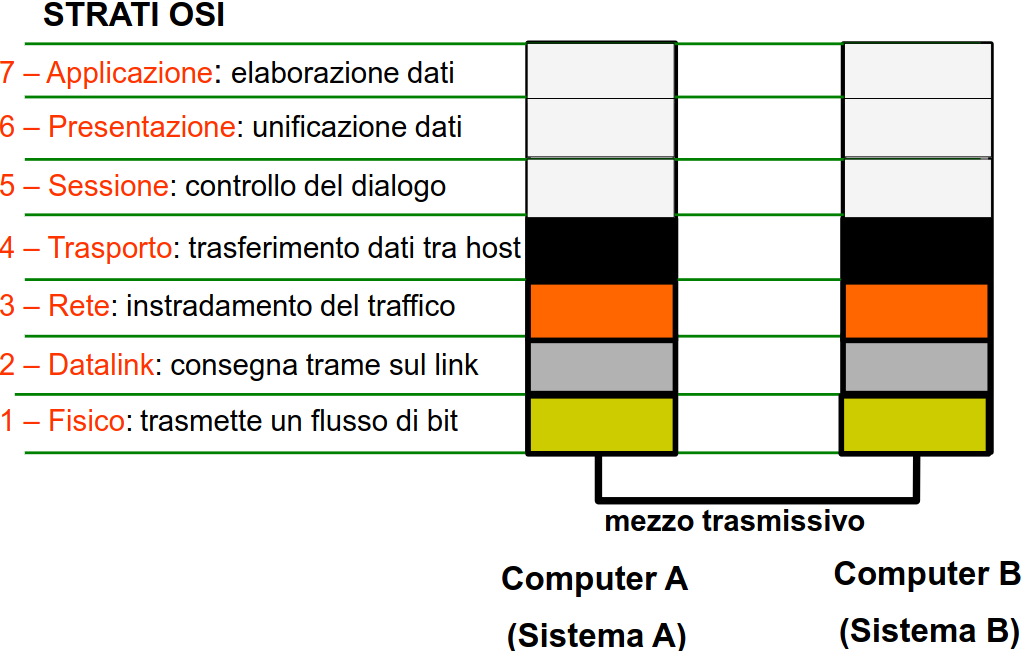
\includegraphics[scale=0.34]{Immagini/Strati_modello_ISO-OSI.png}
    \caption{Strati definiti nel modello ISO/OSI}
\end{figure}
\begin{itemize}
    \item \textbf{\textcolor{purple}{Livello Fisico:}} 
        \begin{itemize}
        \item Comprende tutte le funzioni (procedure meccaniche ed elettroniche) che permettono una connessione a livello fisico.
        \item Si occupa della trasmissione dei bit attraverso il mezzo trasmissivo e delle caratteristiche di cavi e connettori.
        \end{itemize}
    \item \textbf{\textcolor{purple}{Livello di Collegamento:}} 
        \begin{itemize}
            \item Definisce le regole per inviare e ricevere informazioni tra due sistemi in comunicazione.
            \item Si occupa di formare i dati da inviare attraverso il livello fisico, incapsulando i dati in un pacchetto provvisto di header (intestazione) e tail (coda), chiamato frame.
        \end{itemize}
    \newpage
    \item \textbf{\textcolor{purple}{Livello di Rete:}}
        \begin{itemize}
            \item Deve far giungere i “pacchetti” a destinazione.
            \item Si occupa dell’istradamento (“routing”) dei pacchetti, cioè di determinare la sequenza di collegamenti punto-punto necessari per trasmettere un pacchetto da un nodo generico della rete a un altro.
        \end{itemize}
    \item \textbf{\textcolor{purple}{Livello di Trasporto:}}    
        \begin{itemize}
            \item Questo strato fornisce un servizio di trasferimento dati end-to-end.
            \item Si occupa di instaurare, mantenere e terminare una connessione.
            \item Può offrire funzionalità per frammentare e riassemblare i dati, rilevare e correggere gli errori, controllare il flusso dei dati.
        \end{itemize}
    \item \textbf{\textcolor{purple}{Livello di Sessione:}} assembla il dialogo tra nodi in unità logiche.
    \item \textbf{\textcolor{purple}{Livello di Presentazione:}} adatta la sintassi dei dati di ciascuna applicazione alla sintassi richiesta dalla sessione.
    \item \textbf{\textcolor{purple}{Livello di Applicazione:}} protocolli a supporto di applicazioni distribuite.
\end{itemize}

\begin{figure}[h]
    \centering
    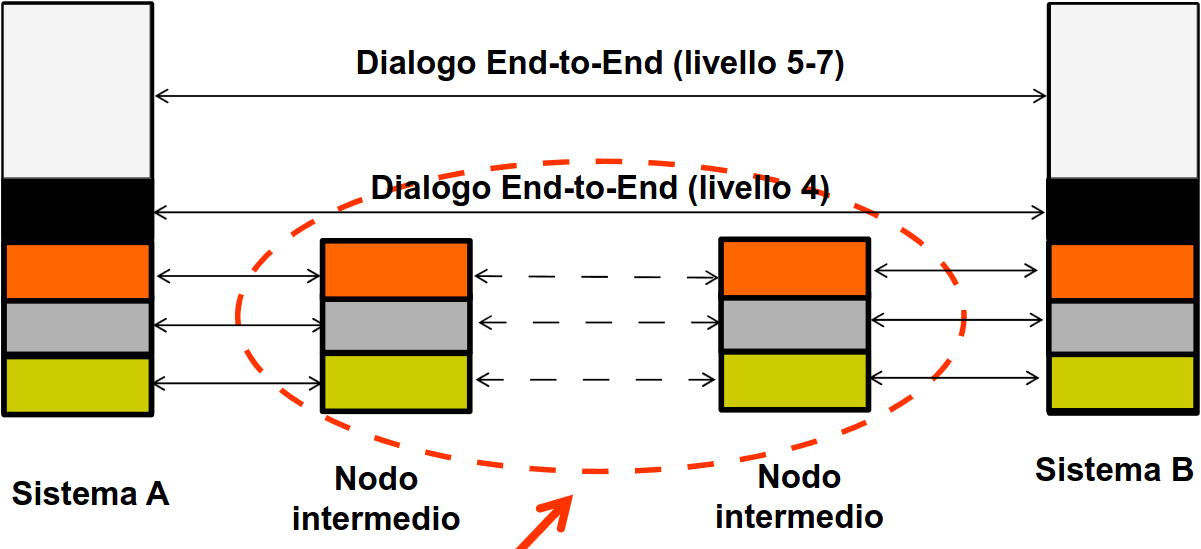
\includegraphics[scale=0.30]{Immagini/Collegamento-End-System.png}
    \caption{Collegamento tra End-System}
\end{figure}

\paragraph{Modalità di Servizio} Esistono due principali metodologie di funzionamento per la comunicazione:
\begin{itemize}
    \item \textbf{\textcolor{purple}{Connection-Oriented:}} 
        \begin{itemize}
            \item Associazione logica tra due o più sistemi al fine di trasferire dati.
            \item Gestione della connessione:
                \begin{itemize}
                    \item Instaurazione della connessione.
                    \item Trasferimento dati.
                    \item Chiusura della connessione
                \end{itemize}
        \end{itemize}
    \item \textbf{\textcolor{purple}{Connection-Less:}} I dati vengono trasferiti senza l'instaurazione di una connessione.
\end{itemize}

\paragraph{Flusso dell'informazione}
Dal punto di vista delle rete, le informazioni hanno tutte origine dal livello Applicativo. L'informazione discende i vari livelli fino alla trasmissione sul canale fisico.
Ogni livello aggiunge all’informazione del livello superiore una propria sezione informativa (o più) denominata header, che contiene informazioni riguardanti esclusivamente quel livello.
\newline Per i dati ricevuti si segue il cammino inverso.

\paragraph{Incapsulamento} Il processo di incapsulamento, ovvero quello nel quale ogni strato aggiunge dell'informazione a quella già presente, è un processo reversibile che garantisce l'estrazione durante la risalita delle informazioni dal livello di rete al livello applicativo (o fino ad un livello inferiore se ci troviamo in un nodo intermedio).
\newline In questo processo abbiamo:
\begin{itemize}
    \item \textcolor{purple}{Header:} Contente informazioni relative a quel livello.
    \item \textcolor{purple}{Payload:} Dati provenienti dal livello superiore.
    \item \textcolor{purple}{Tail:} Generalmente utilizzato per l'individuazione e la correzione degli errori.
\end{itemize}
\newpage
\begin{figure}[h]
    \centering
    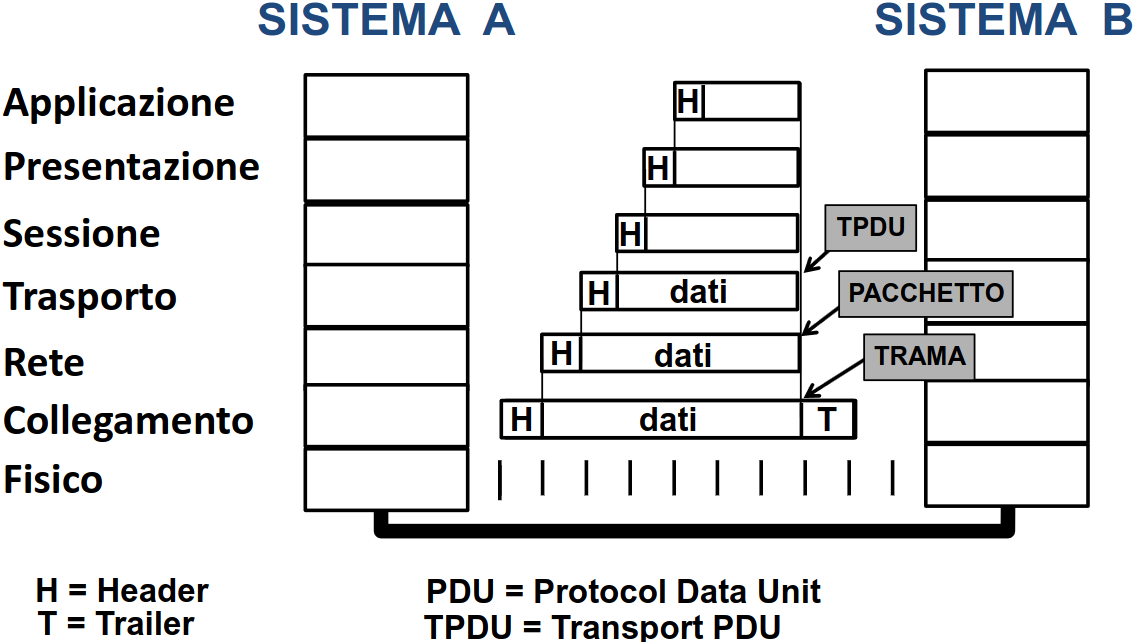
\includegraphics[scale=0.30]{Immagini/Incapsulamento-dati.png}
    \caption{Processo di incapsulamento}
\end{figure}

\subsection{Stack TCP/IP}
TCP/IP è una famiglia di protocolli attualmente utilizzata in Internet. Si tratta di una gerarchia di protocolli, ciascuno dei quali fornisce funzionalità specifiche.
\newline Definita in origine in termini di quattro livelli software soprastanti a un livello hardware, la pila TCP/IP è oggi intesa come composta di cinque livelli.
\begin{itemize}
    \item \textbf{\textcolor{purple}{Applicazione:}} supporta le applicazioni di rete, collegamento logico end-to-end; scambio di messaggi tra due processi (ftp, smtp, http).
    \item \textbf{\textcolor{purple}{Trasporto:}} trasferimento dati end-to-end da un host sorgente all’host destinatario (Tcp, Udp).
    \item \textbf{\textcolor{purple}{Rete:}} instradamento dei datagrammi dalla sorgente alla destinazione (Ip, ICMP).
    \item \textbf{\textcolor{purple}{Link:}} trasferimento dati in frame attraverso il collegamento tra elementi di rete vicini (Point-to-Point Protocol, Ethernet, ...).
    \item \textbf{\textcolor{purple}{Fisico:}} trasferimenti dei bit di un frame sul mezzo trasmissivo.
\end{itemize}

\newpage

\paragraph{Differenze tra ISO/OSI e TCP/IP} Nella pratica in Internet viene utilizzato lo stack protocollare TCP/IP. Questo accade perché ISO/OSI, a differenza di TCP/IP, fornisce una specifica generale, difficile da implementare e poco efficiente. ISO/OSI però viene utilizzato ancora come modello di riferimento.